\title{Esercitazione 6 30/04/2020}\newline
\textbf{link} \href{https://web.microsoftstream.com/video/e7731d3b-34c1-4fd2-a49a-606e7413fb96}{Clicca qui}
\section{Esercitazione VI}
\url{../esercitazione6/pdf/06-Statica02.pdf}\newline
\url{../esercitazione6/pdf/ese_6_notes.pdf}
\subsection{Forza elastica}
Data una molla con lunghezza indeformata $l_0$ e costante elastica $k$, e una forza $F_e$ applicata su di essa\newline
[immagine dagli appunti del prof]
\begin{center}
    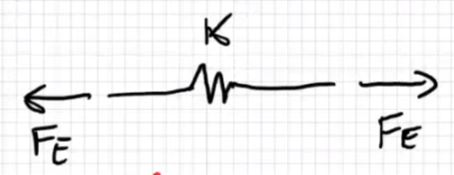
\includegraphics[height=3cm]{../esercitazione6/img1.JPG}
\end{center}
allora la deformazione ottenura è pari a $\Delta l = \frac{F_e}{k}$, oppure, al contrario, a fronte di una deformazione $\Delta l = l - l_0$, la molla avrà un richiamo elastico pari a $F_e = k \Delta l$.\newline
\newline
Se $\Delta l > 0$ allora la molla è in trazione e di conseguenza avremo un allungamento, invece, se $\Delta l < 0$ la molla è in compressione e avremo quindi un accorciamento.\newline
\newline
Per risolvere gli esercizi, si può eliminare una molla e sostituirla con la sola forza $F_e$ applicata ai suoi estremi.
\subsection{Forza applicata su un vincolo}
Se ci ritroviamo nella situazione in cui un forza esterna viene applicata a un vincolo che collega due corpi rigidi, bisogna capire come questa viene distribuita sui due corpi.\newline
\newline
Per farlo è sufficiente slegare e studiare in maniera indipendente i due corpi (introducendo le forze del vincolo), ma anche il vincolo (introducendo le forze del vincolo). A questo punto utilizzando le equazioni cardinali della statica sul vincolo e sui corpi si può determinare il valore delle forze vincolari per i due corpi e quindi dedurre la distribuzione sui due corpi della forza originariamente applicata al vincolo.
\subsection{Biella}
Una biella, se non ha forze applicate lungo l'asta, ha azione di taglio e momento flettente nulli.